\chapter{Implementierung der Karte}
\label{chap:3}

\begin{wrapfigure}{R}{0.5\textwidth}
	\vspace{-\baselineskip}
	\centering
	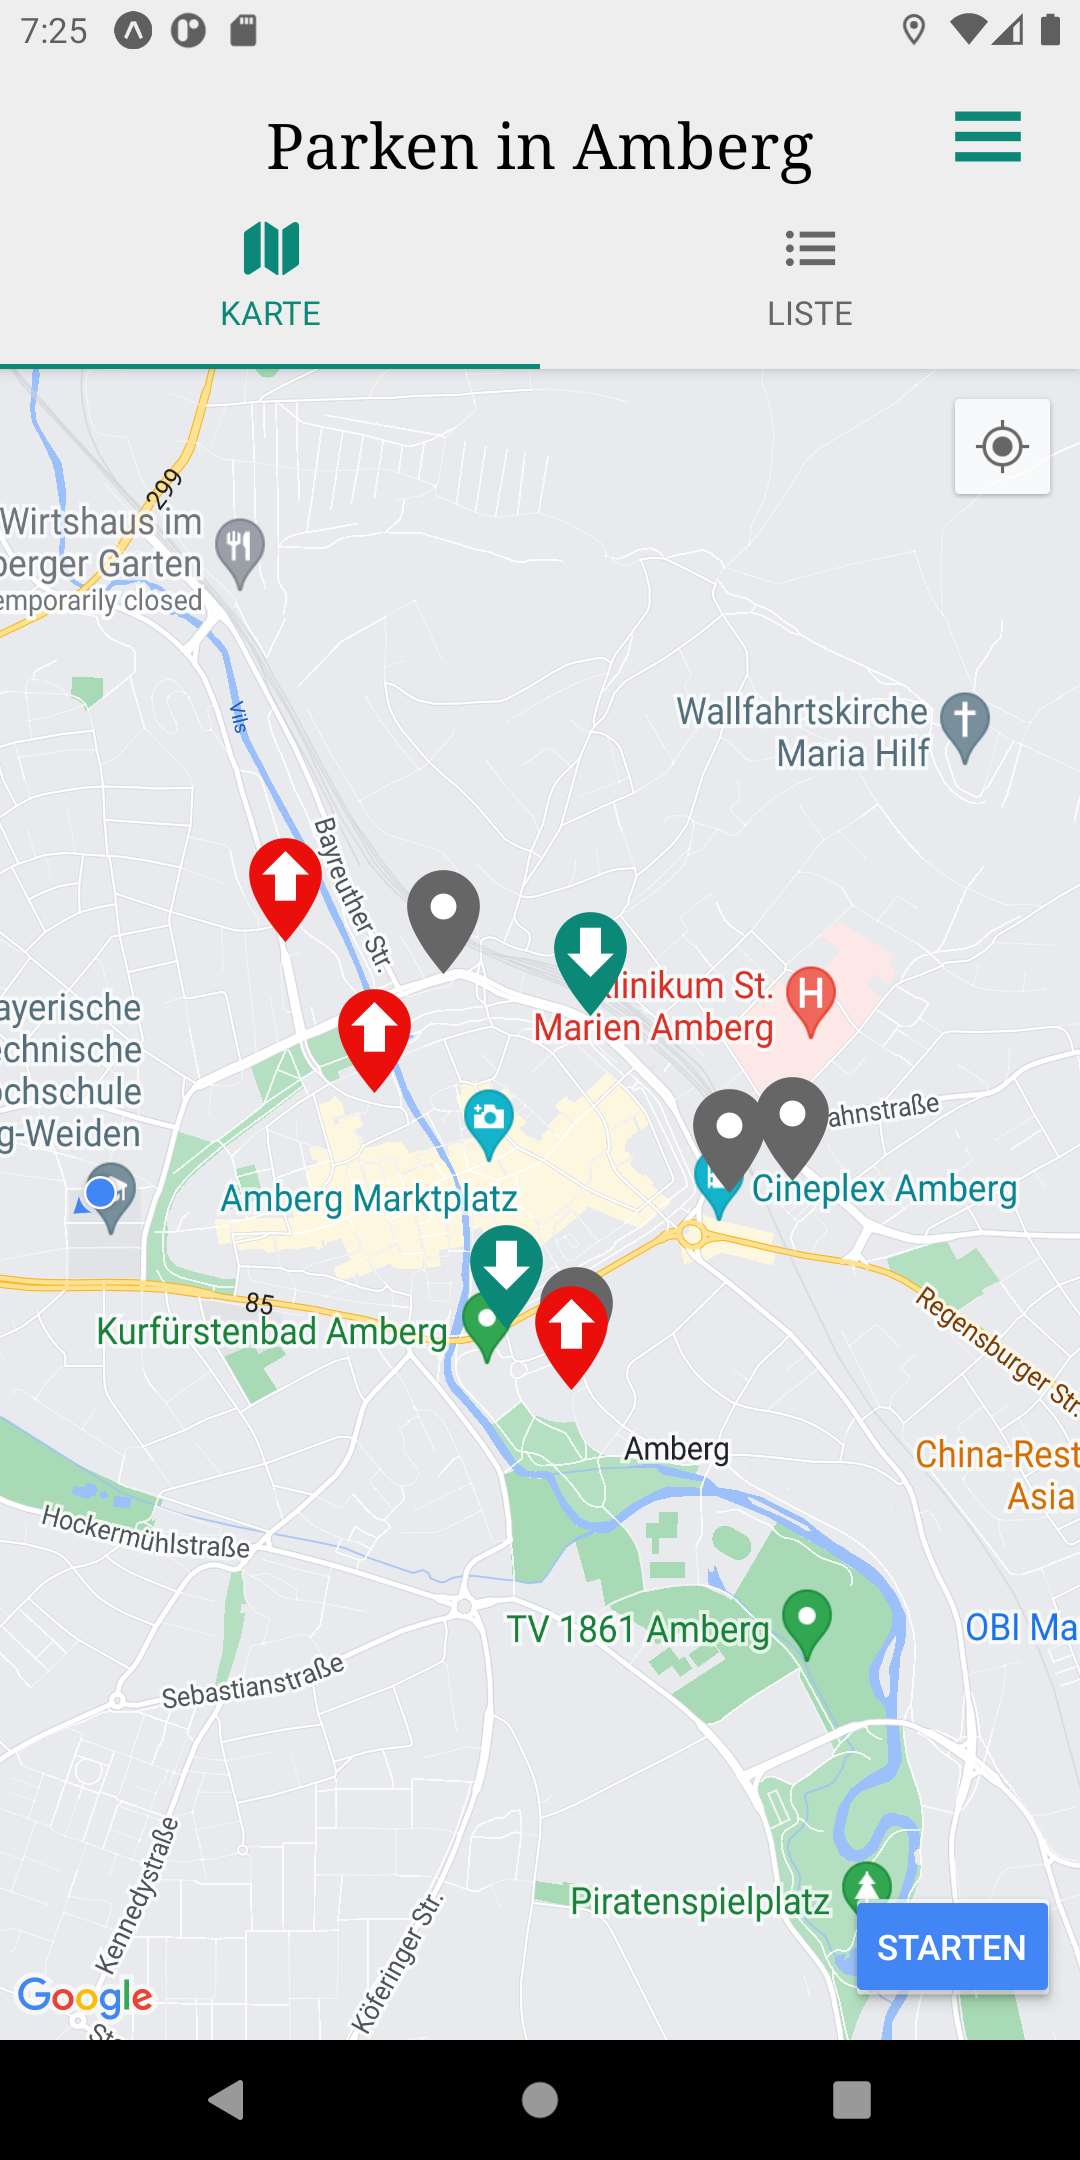
\includegraphics[scale=0.15]{img/map}
	\caption{Ansicht der fertigen App mit der Karte und eingezeichneten Markern}
	\label{fig:map}
\end{wrapfigure}
Die Karte und alle Zusatzfunktionalitäten sind im Ordner \verb|Map| zu finden. Ein erster Prototyp der Karte war sehr schnell implementiert. Hierfür musste nur das Paket react-native-maps installiert werden \cite{maps}. Dieses Paket benutzt auf Android-Systemen die Google Maps API und auf iOS-Systemen die Apple Maps API, um eine Karte in der App anzeigen zu können. Wenn dieses Paket mit Expo installiert wird, sind sogar keine API-Keys nötig, um die Karten anzeigen und nutzen zu können. Um nun auch den Standort des Nutzers in der Karte zeigen zu können, wird das Expo-Paket expo-location benötigt \cite{location}. Dieses Paket kann, wenn der Nutzer die Erlaubnis gibt, den Standort des Nutzers herausfinden und in die Karte einzeichnen. Wenn der Nutzer seine Erlaubnis nicht gibt, wird dies auch wahrgenommen und die Funktionalität der App ist dadurch eingeschränkt, da dann nicht mehr herausgefunden werden kann, wie nah der Nutzer einem Parkhaus ist. Um die Parkhäuser in die Karte einzuzeichnen wurde eine Liste aus den statischen Daten erzeugt, welche an das react-native-maps Paket übergeben wird.

Diese Markierungen der Parkhäuser wurden danach noch mit Icons versehen, welche den Trend anzeigen. Diese Icons stammen aus dem react-native-vector-icons Paket \cite{vector-icons}. Die Icons aus diesem Paket werden in der gesamten App verwendet. Ein grüner Marker mit einem Pfeil nach unten bedeutet, dass sich das Parkhaus gerade leert. Ein roter Marker mit einem Pfeil nach oben heißt, dass sich das Parkhaus füllt. Ein grauer Marker bedeutet, dass das Parkhaus einen gleichbleibenden Trend besitzt. Somit kann der Nutzer schon beim Starten der App sofort Informationen zu den Parkhäusern auslesen. Diese Marker mit der Karte sind in \autoref{fig:map} zu sehen. Hier ist der Nutzer als kleiner blauer Punkt mit einem Pfeil in Blickrichtung bei der OTH eingezeichnet.

\begin{wrapfigure}{R}{0.5\textwidth}
	\vspace{-\baselineskip}
	\centering
	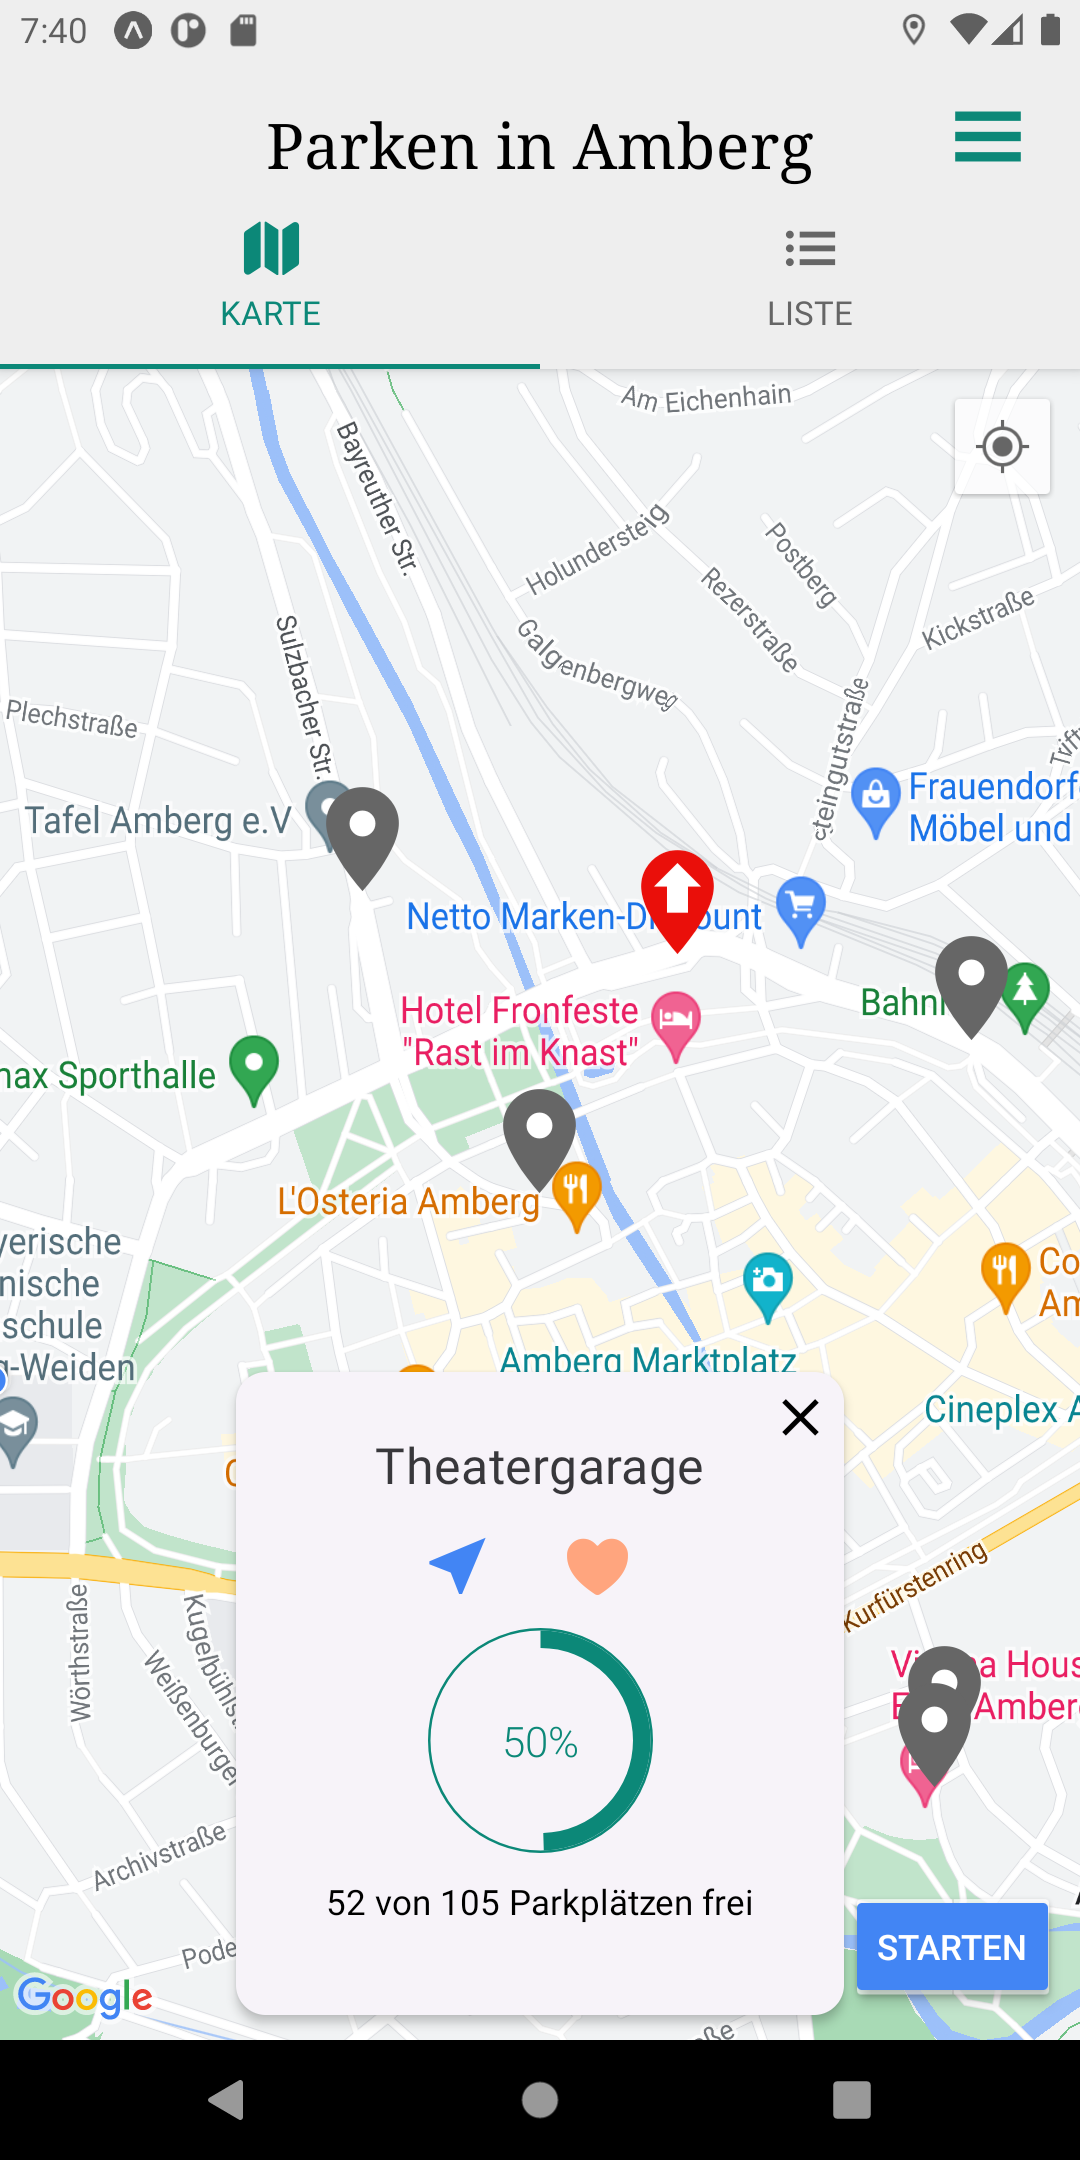
\includegraphics[scale=0.15]{img/detail_map}
	\caption{Detailansicht zum Parkhaus Theatergarage in der Karte}
	\label{fig:detail_map}
\end{wrapfigure}
Durch Anklicken der Marker ist es auch möglich, nähere Informationen zu den einzelnen Parkhäusern zu bekommen. Diese Ansicht ist in \autoref{fig:detail_map} zur Theatergarage zu sehen. Hier wird angezeigt, wie viele Plätze in diesem Parkhaus noch frei sind. Zur besseren Benutzerfreundlichkeit wird dies noch mit einem Fortschritts-Kreis visualisiert, welcher aus dem react-native-progress Paket stammt \cite{progress}. Dieser zeigt den Füllstand des Parkhauses in Prozent an. Je größer der Prozentwert, desto mehr Parkplätze sind frei. Über diesem Kreis sind zwei Icons zu sehen. Der blaue Pfeil links bedeutet die Navigation. Durch Klicken auf dieses Icon wird der Nutzer zu diesem bestimmten Parkhaus navigiert, was später erläutert wird. Das rote Herz rechts bedeutet, dass dieses Parkhaus vom Nutzer zu den Favoriten hinzugefügt wurde. Wenn das Parkhaus nicht zu den Favoriten gehört, ist das Herz nicht ausgefüllt. Durch einen Klick auf dieses Icon kann der Nutzer zudem das Parkhaus zu den Favoriten hinzufügen oder wieder entfernen.

\begin{wrapfigure}{R}{0.5\textwidth}
	\vspace{-\baselineskip}
	\centering
	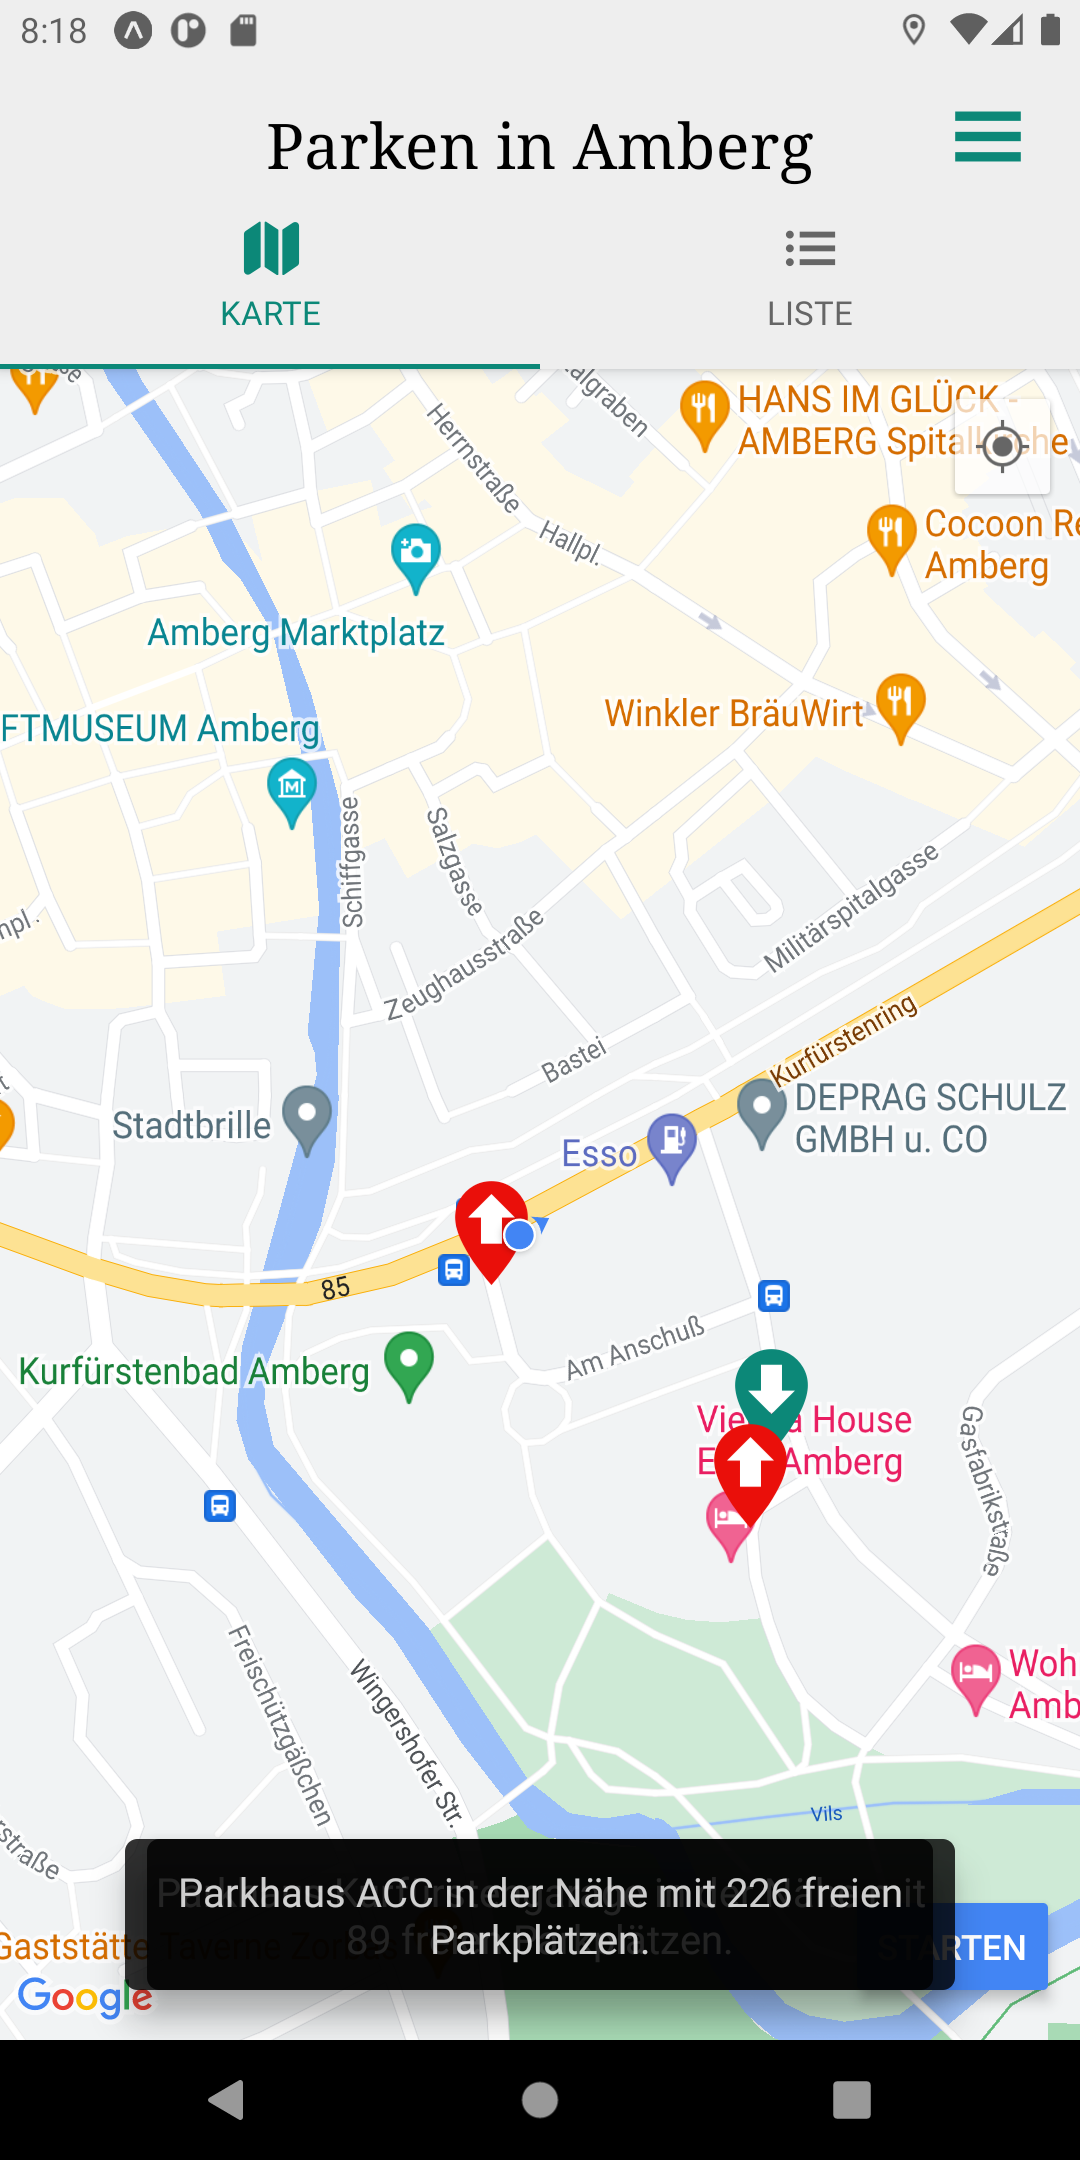
\includegraphics[scale=0.15]{img/Geofencing}
	\caption{Anzeige, dass sich der Nutzer dem Parkhaus ACC nähert, welches 226 freie Parkplätze hat}
	\label{fig:Geofencing}
\end{wrapfigure}
Nachdem die Karte fertig implementiert war, konnten die Anzeigen erstellt werden, dass sich der Nutzer einem Parkhaus nähert. Dies wurde zuerst über Geofencing versucht zu lösen. Geofencing bedeutet, dass die App kreisförmige Bereiche, welche für den Nutzer meist nicht sichtbar sind, um Koordinaten aufspannt. Bei Betreten und Verlassen eines dieser Bereiche wird ein Event mit den Informationen zu dem Bereich, also hier dem Parkhaus, gefeuert. Im expo-location Paket ist standardmäßig Geofencing enthalten. Dies wurde versucht einzufügen, jedoch kam es hierbei zu Problemen. Wenn der Nutzer in mehreren Geofences ist, kann es passieren, dass das Betreten eines anderen Geofences doppelt signalisiert ist. Wie in \url{https://github.com/expo/expo/issues/6283} zu sehen, besteht dieses Problem immer noch und es scheint keinen Fix hierfür zu geben. Deshalb wurde ein eigenes Geofencing implementiert, welches im Ordner \verb|Geofencing| zu finden ist. Dafür musste die Luftlinienentfernung vom Nutzer zu jedem Parkhaus berechnet werden, ob er in der Nähe eines Parkhauses ist. Zur Berechnung der Distanz wurde die Haversine Formel verwendet \cite{haversine}. Diese kann über die Umwandlung der Winkelkoordinaten Latitude und Longitude ins Bogenmaß den Abstand zwischen zwei Punkten auf einer Kugel berechnen.

Um nun den Abstand zu den Parkhäusern zu berechnen, wurde die Position des Nutzers benötigt. Dafür existiert wieder eine Funktion in expo-location, nämlich \verb|startLocationUpdatesAsync|. Diese Funktion schickt kontinuierlich die aktuellen Koordinaten des Nutzers an einen Task, der vorher definiert wurde und im Hintergrund läuft. Tasks können mithilfe des expo-task-manager Pakets gestartet werden \cite{task}. Der Task nimmt die Koordinaten an und übergibt diese an eine Funktion, welche den Abstand dieser Koordinaten zu jedem Parkhaus berechnet. Falls der Abstand kleiner als 200 Meter ist, wird der Nutzer als ,,in der Nähe des Parkhauses'' angesehen. Falls der Nutzer vorher weiter entfernt als 200 Meter vom Parkhaus war, also außerhalb des ,,Geofences'', erscheint ein Meldung als Toast durch das react-native-root-toast Paket \cite{toast}, welchem Parkhaus der Nutzer sich gerade nähert und wie viele freie Parkplätze in diesem aktuell sind. Diese Meldung wird auch über das expo-speech Paket vom Smartphone vorgelesen \cite{tts} und ist die einzige, die zudem vorgelesen wird. Alle anderen werden nur über Toasts gezeigt. Die graphische Anzeige der Meldung ist in \autoref{fig:Geofencing} ersichtlich. In welchen Geofences der Nutzer gerade ist, wird in einer Liste festgehalten, die später benötigt wird.

\begin{wrapfigure}{R}{0.5\textwidth}
	\vspace{-\baselineskip}
	\centering
	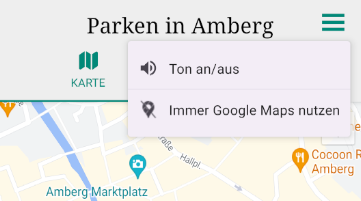
\includegraphics[scale=1]{img/map_settings}
	\caption{Liste an Einstellungen der Karte, welche über ein Burger-Menü verfügbar ist}
	\label{fig:map_settings}
\end{wrapfigure}
Zuletzt wurde die Karte noch mit zwei Einstellungsmöglichkeiten konfigurierbar gemacht. Diese sind über das Burger-Menü rechts oben aufrufbar. Bei Klicken auf das Menü öffnet sich eine Liste mit zwei Einträgen, wie in \autoref{fig:map_settings} sichtbar. Dieses Menü stammt aus dem Paket react-native-paper \cite{paper}. Der erste Eintrag des Menüs steuert, ob die Meldung, dass ein Geofence betreten wurde, vorgelesen werden soll oder nicht. Wenn das Icon des Lautsprechers durchgestrichen ist, wird die Vorlese-Funktion ausgeschaltet. Standardmäßig ist diese Funktion angeschaltet. Der zweite Eintrag gibt an, ob bei der Navigation ausschließlich zu Google Maps weitergeleitet werden, oder ob die interne Navigation der App, wenn möglich, genutzt werden soll. Auf diese Navigation wird in \autoref{chap:5} weiter eingegangen. Diese Einstellung ist standardmäßig ausgeschaltet, damit die interne Navigation bevorzugt wird. Die Werte beider Einstellungen werden zudem ebenfalls in async-storage gespeichert, damit der Nutzer die App nicht bei jedem Öffnen neu konfigurieren muss.

Damit ist die Implementierung der Karte abgeschlossen. Im Folgenden wird die Funktionalität und Umsetzung der Liste beschrieben.
